\documentclass{article}
\usepackage{graphicx}

\begin{document}
\title{Requirements Specification Document}
\author{Team D}
\date{\today}

\maketitle

\vspace*{1.5in}
\begin{table}[htbp]
\caption{Team}
\begin{center}
\begin{tabular}{|r | c|}
\hline
Name & ID Number \\
\hline\hline
Stefanie Lavoie & 1951750 \\
Pinsonn Laverdure & 9684352 \\
Ghislain Ledoux & 6376320 \\
Rigil Malubay & 6262732 \\
Philippe Milot & 9164111 \\
Christopher Mukherjee & 6291929 \\
\hline
\end{tabular}
\end{center}
\end{table}

\clearpage

\section{Introduction} % Status: COMPLETE

This document will describe in detail the requirement specifications for the Vessel Monitoring System which is to be developed in the context of the COMP354 course. The requirements specifications include an overview of the system and its goals, a detailed description of all functional and non-functional requirements (modeled using Use Case Diagrams and Domain Model Diagrams), as well as a development plan. 

If a requirement appears in this document, the final Vessel Monitoring System \emph{must} conform to this requirement. Inversely, the Vessel Monitoring System is not required to conform to any other requirement that is not specified in this document.

\section{Project Description} % Status: COMPLETE

The Vessel Monitoring System is a Java-based system which listens to incoming radar data from multiple vessels at sea and keeps track of their type, position, and velocity. The goal of the system is to ensure that no vessels ever collide with one another.

To accomplish this, the system tracks ``risk zones'' around each tracked vessel. The \emph{Low-Risk Zone} is defined as the circle area with a 200m radius around the vessel. The \emph{High-Risk Zone} is defined as the circle area with a 50m radius around the vessel. The system shall generate appropriate alarms when a dangerous situation arises, e.g. when two vessels' risk zones start to overlap. The system will issue a \emph{Low-Risk Alert} whenever two or more Low-Risk Zones overlap. The system will issue a \emph{High-Risk Alert} whenever two or more High-Risk Zones overlap.

The VMS has a graphical desktop application component. Radar data is visually accessible at all times in two different modes:

The \emph{List Mode} presents a list of all currently-tracked ships. Each row in the list contains all known metadata associated with a single ship: The Vessel ID, the Type, the X-Y coordinates, the Speed (in m/s), the Course, the Distance from starting point, and the time and date of last-received data. The list can be sorted by any of its columns, in both ascending and descending orders.

In this mode, the alerts are represented by highlighting the rows of the vessels involved in the alert. A Low-Risk Alert will highlight the rows in yellow. A High-Risk Alert will highlight the rows in red.

\begin{figure}[h]
\caption{A sketch of the user interface}
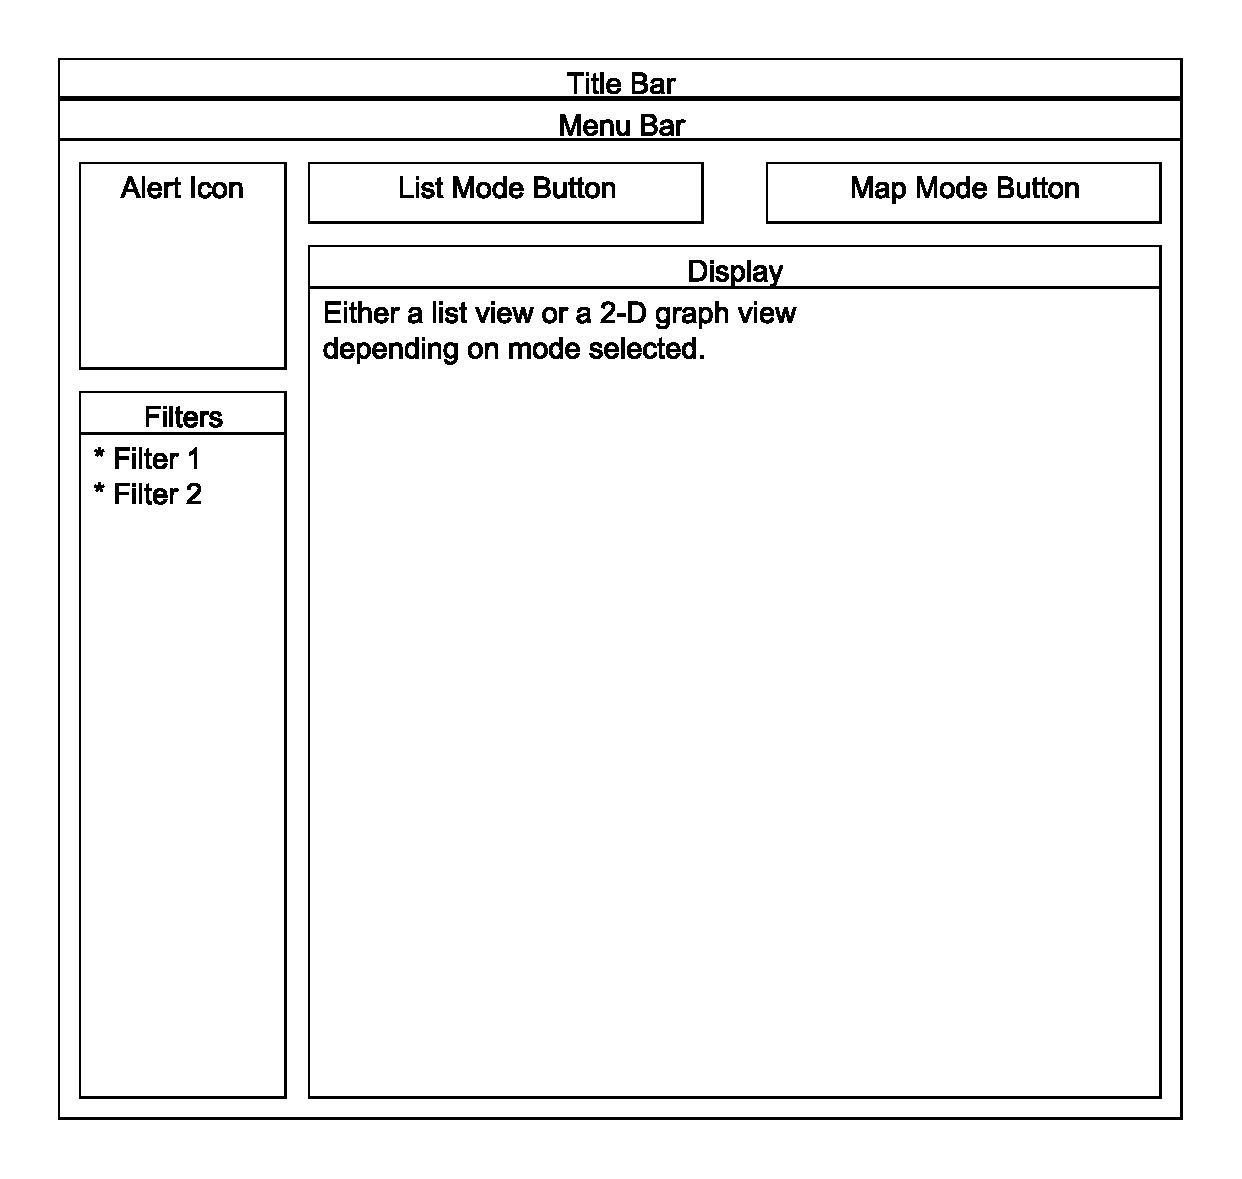
\includegraphics[width=\linewidth]{gui-proto.eps}
\end{figure}

The \emph{Map Mode} displays a 2-D grid where each tracked vessel is represented as a dot placed on the grid according to its X-Y coordinates. The colour of the dot represents the Vessel Type. Additionally, two wider circles around each dot represent the vessel's two ``risk zones''. The Low-Risk zone is displayed as a circle of 200m around the ship. The High-Risk zone is displayed as circle of 50m.

In this mode, the alerts are represented by colour-coding the circles. When two ships have overlapping Low-Risk Zones, the circles will turn yellow. When two ships have overlapping High-Risk Zones, the circles will turn red.

Both view modes update the display in real-time, at a refresh rate which is configurable by the user. Both views can be filtered by Vessel Type. Both views display an ``Alert Icon'' in the top-left corner of the window. This icon is a large, white number against a colored background. The number represents how many alerts are currently in effect. The background color represents the severity of the highest-risk alert currently in effect (red for High-Risk, yellow for Low-Risk, green when no alerts are in effect).

\subsection{Vessel Simulator}

For the sake of testing, the system will also include a \emph{Vessel Simulator} which will emulate the behavior of a real vessel. The Simulator is a simple command-line utility which will read vessel data from a file, connect to the VMS, and periodically send updated vessel data to the VMS.

The format of the file is that of a standard VSF file. The description of the format is beyond the scope of this document.

\break
\section{Goals and Constraints} % Status: See subsections.

\subsection{Functional Requirements} % Status: Need to incorporate UCDs from Stefanie and Pinsson.

\begin{figure}[h]
\caption{Vessel Monitoring System Use Case Diagram}
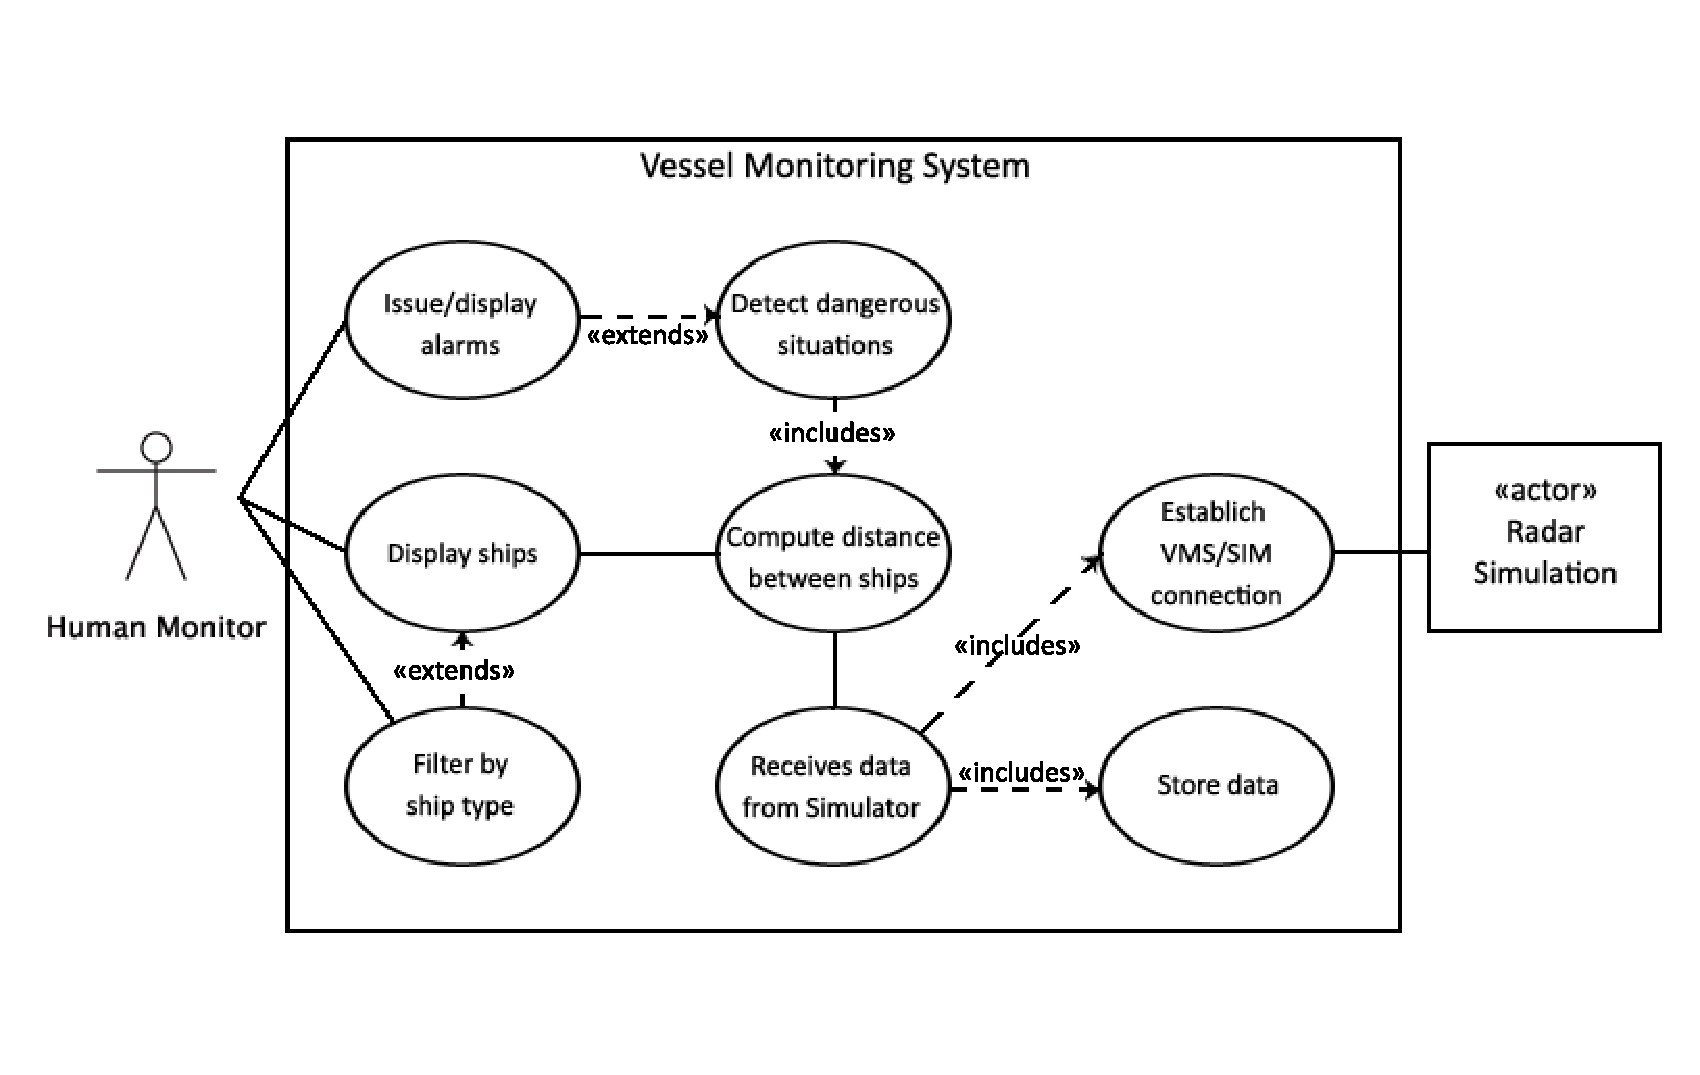
\includegraphics[width=0.8\textwidth]{vmsdiagram.eps}
\end{figure}

\subsubsection{Use Case 1} \label{uc:1}

\noindent
{\bf Name}\\
Vessel Monitoring System - Normal State

\noindent
{\bf Summary}\\
The Vessel Monitoring System is used to show the location of various vessels on a map. This Use Case scenario explains what happens when the Vessel Monitoring System is operation normaly without any alert or problems.

\noindent
{\bf Actors}\\
User, Monitoring System and Radar Simulation.

\noindent
{\bf Precondition}\\
A new ship is ready to send data from the Radar Simulation to the Monitoring System.

\noindent
{\bf Main Scenario}\\
\vspace*{-0.2in}
\begin{enumerate}
\item User open the monitoring system program to check vessel locations.
\item Monitoring System establish a connection with the Radar Simulation.
\item Radar Simulation sends new information to Vessel Monitoring System.
\item Vessel Monitoring System obtains the new information from the Radar Simulation and stores the data.
\item Vessel Monitoring System updates the information shown on the User's screen.
\item User can filter through different types of vessels and select the ones they want to display.
\item Monitoring system displays only the vessels choosen by the user.
\item User closes the Vessel Monitoring System program.
\end{enumerate}

\noindent
{\bf Exceptions}\\
Vessel Monitoring System is not receiving the data from the Radar Simulation and cannot display the vessels.

\noindent
{\bf Postcondition}\\
\vspace*{-0.2in}
\begin{enumerate}
\item The Vessel Monitoring System receives and store the data correctly and the ship's position is updated on the screen.
\item The System is now waiting for new data to arrive.
\end{enumerate}

\noindent
{\bf Priority}\\
1

\noindent
{\bf Traces to Test Cases}\\
Add when test cases done.

\subsubsection{Use Case 2} \label{uc:2}

\noindent
{\bf Name}\\
Vessel Monitoring System - Alert State

\noindent
{\bf Summary}\\
The Vessel Monitoring System is used to show the location of various vessels on a map. This Use Case scenario explains what happens
when the Vessel Monitoring System needs to display an alert because the distance between two or more vessels is too short.

\noindent
{\bf Actors}\\
User, Monitoring System and Radar Simulation.

\noindent
{\bf Precondition}\\
A new ship is ready to send data from the Radar Simulation to the Monitoring System and two ships are too close to each other.

\noindent
{\bf Main Scenario}\\
\vspace*{-0.2in}
\begin{enumerate}
\item User open the monitoring system program to check vessel locations.
\item Monitoring System establish a connection with the Radar Simulation.
\item Radar Simulation sends new information to Vessel Monitoring System.
\item Vessel Monitoring System obtains the new information from the Radar Simulation and stores the data.
\item Vessel Monitoring System updates the information shown on the User's screen.
\item Vessel Monitoring System detects that two ships are near each other and displays an alert.
\item User closes the Vessel Monitoring System program.
\end{enumerate}

\noindent
{\bf Exceptions}\\
Vessel Monitoring System is not receiving the data from the Radar Simulation and cannot display the vessels.\\
The vessels are not near each other enough to create an alert.

\noindent
{\bf Postcondition}\\
\vspace*{-0.2in}
\begin{enumerate}
\item The Vessel Monitoring System receives and store the data correctly and the ship's position is updated on the screen.
\item The Vessel Monitoring System hides the warning once the threat is gone.
\item The System is now waiting for new data to arrive.
\end{enumerate}

\noindent
{\bf Priority}\\
1

\noindent
{\bf Traces to Test Cases}\\
Add when test cases done.


\subsubsection{ Radar Simulator Use Cases}
\begin{figure}[h]
\caption{Radar simulator Use Case Diagram}
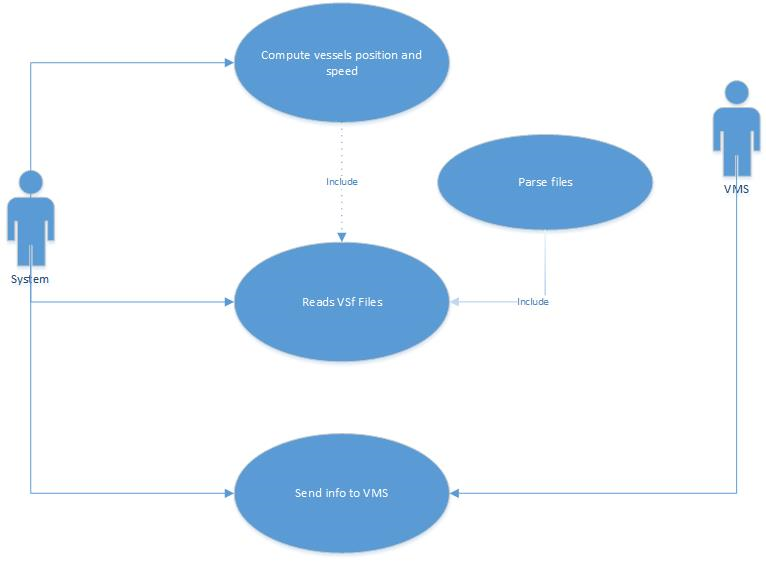
\includegraphics[width=1.0\textwidth]{usecasediagram}
\end{figure}

\noindent
{\bf Name}\\
Radar simulation -Normal Running process

\noindent
{\bf Actors}\\
Vessel monitoring system, Java system

\noindent
{\bf Goals}\\
To send valid vessel information to the VMS

\noindent
{\bf Preconditions }\\
A vsf  file is created and placed in the required locations. 
The file has information on different vessels.

\noindent
{\bf Summary }\\
The radar simulator will read the locations of different types of vessel in a range of 5000 meters,
compute the locations and directions of each vessels, send the different information to the vessel monitoring system, and update every time the vessels change position or location.

\noindent
{\bf steps }\\ 
\begin{enumerate}
\item Open and read the vsf file 
\item Validate the vsf files by checking that there is valid information in the file 
\item Read each line of the file 
\item Disregard any comments that are found in the file
\item Calculate the speed, location, directions, etc.
\item Send the information to the VMS.
\item Repeat steps three to six until the entire file has been read
\item Close the file and quit
\end{enumerate} 

\noindent
{\bf Name}\\
Radar simulation - File not valid 

\noindent
{\bf Actors}\\
Java system 

\noindent
{\bf Goals}\\
To open the vsf file and make sure that it is valid 

\noindent
{\bf Preconditions }\\
A vsf file is created and placed in the required locations.

\noindent
{\bf Summary }\\
The radar simulator will read the locations of different types of vessel in a range of 5000 meters,
compute the locations and directions of each vessels, send the different informations to the vessel monitoring system, update every time the vessels change position or location.

\noindent
{\bf steps }\\
\begin{enumerate}
\item Open the vsf file 
\item Try (and fail) to read the vsf file 
\item Stop the radar simulator and send File Not Found Exception 
\end{enumerate} 


\subsection{Domain Model} % Status: Need to create domain model diagram.

\begin{figure}[h]
\caption{VMS Domain Model Diagram}
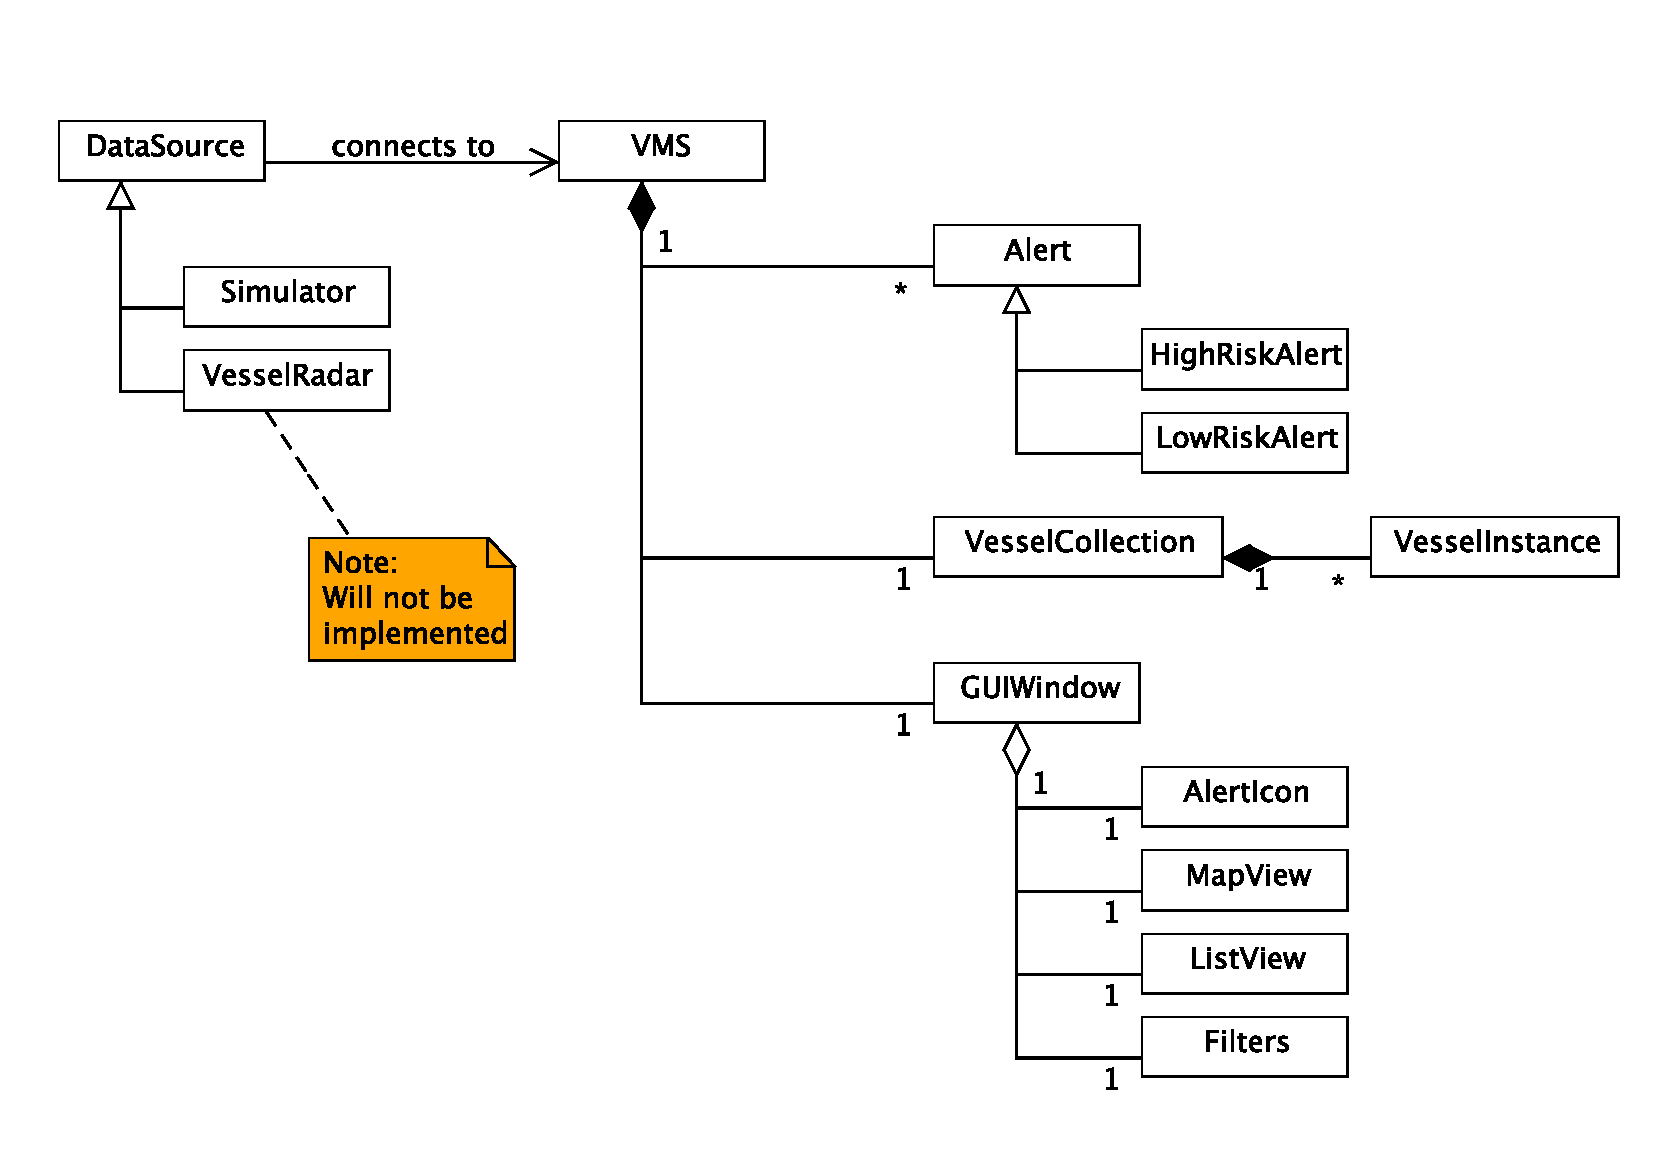
\includegraphics[width=\linewidth]{domain-model.eps}
\end{figure}

\begin{figure}[h]
\caption{Radar Simulator Domain model}
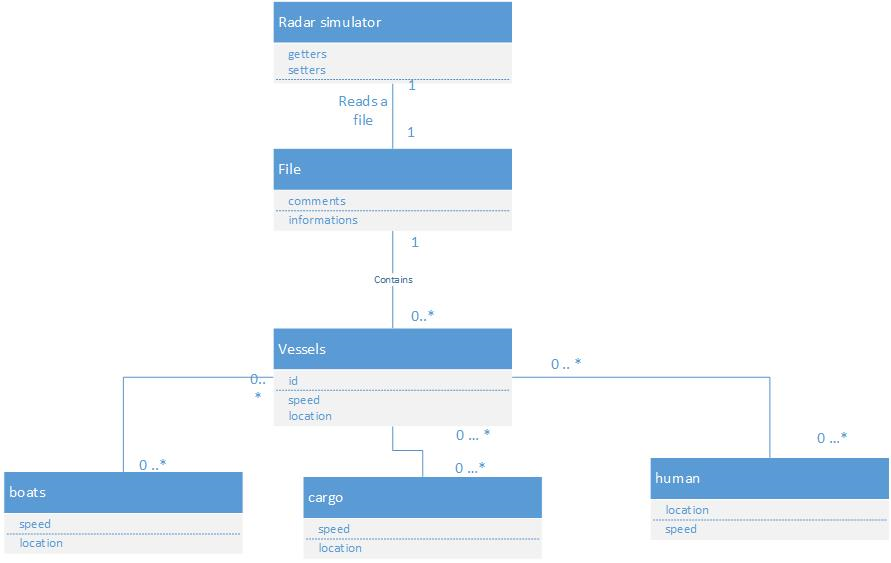
\includegraphics[width=\linewidth]{DMusecase}
\end{figure}

\subsection{Constraints} % Status: Satisfactory, but can keep adding as they are thought up.

\subsubsection{Shared constraints}
Both applications shall run on Windows 7 or later, and Mac OS X 10.7 or later.

Both applications shall require the Java 7 platform to run.

\subsubsection{VMS constraints}
Functionally, the VMS shall be limited to keeping track of 100 unique ships at any time. This is to avoid slowdown as the number of ships increase. If new data comes in that pushes the number of unique ships over that limit, the VMS shall ``forget'' the oldest ship already tracked to make room for the new one, and issue a warning to the human operator.

\subsubsection{Simulator constraints}

No user interface shall be designed for the Simulator. It is strictly a separate command-line tool.

If a VSF file has a timestep of less than 0.5 (which is the minimum accepted timestep), the program will read the file and automatically change the timestep to 0.5.

\section{Resource Evaluation} % Status: See subsections.

\subsection{Human Resources} % Status: Need Pinsson's description. Add availabilities.

\emph{Pinsson Laverdure} has experience with Java mostly in school. He has work as a beta tester for Netgear and will contribute to testing.

\emph{Stefanie Lavoie} has experience with developing on the Java platform (but not using the Swing library for GUI), as well as managing a project's source code using the Git DVCS. Although she has never used \LaTeX before, she will be able to contribute significantly to the design and code of the project.

\emph{Ghislain Ledoux} has a good conciliatory nature which lends itself well to working in teams. He has a good instinct for identifying use cases, which will be useful in the first stages of design. He has no prior experience working with a source control system nor with \LaTeX.

\emph{Rigil Malubay} has good analytical and problem-solving skills. He has prior work experience as a web developer in PHP. According to himself, he lacks attention to detail, but this weakness is mitigated when working closely in a team.

\emph{Philippe Milot} has previous work experience with developping on a wide range of platforms and programming languages (C/C++, Java, Haskell, Perl, Python, PHP, \LaTeX, etc.), which will be useful for informing the technological choices that will be made for the project. He is familiar with Subversion and Git VCS. He has never worked with a Java GUI toolkit before.

\emph{Christopher Mukherjee} has experience with the Java platform as well as web programming. He has previous work experience with tech companies such as Trendex Information Systems and Ericsson. His experience with working in larger teams will help the project reach its deadlines on time. He has never worked with a source control system or with \LaTeX before.

\subsection{Technical Resources} % Status: COMPLETE

The project can make use of the software that is available in the computer labs of Concordia University. 

The project shall be developed in parallel on both Windows and Mac OS X platforms. Development can be done either on Concordia University's computers or the personal computers of the developers.

The project shall be developed on the Java platform version 7. All graphical user interfaces shall use the Swing library.

The project shall use Git as its source-control solution. GitHub shall be used for hosting the repository online.

The project shall use \LaTeX for typesetting all its documentation. Visio and UMLet shall be the tools used to create diagrams.

\section{Scoping} % Status: COMPLETE
The VMS shall not use a separate client/server architecture. The ``server'' part will be directly integrated into the desktop application. The Simulator (and other theoretical vessels) will have to connect to the desktop application to send their data.

Connection issues between the VMS and vessels shall be handled in the most basic way possible (display error message and exit).

No UI shall be provided to customize the limit of a 100 unique ships. Instead, the limit shall be configurable via a command-line argument when starting the VMS. 

No UI shall be provided to customize the address at which the VMS will listen to incoming data. Instead, the limit shall be configurable via a command-line argument when starting the VMS.

\section{Plan} % Status: To be done

\subsection{Activities}

\emph{Software Design Document}: Describes the software architecture of the VMS and Simulator. Written in \LaTeX. 

\emph{Simulator program}: Self-contained program which acts as a fake datasource for the VMS.

\emph{Communication module}: Java code that handles the communication between the VMS and its data sources (such as the Simulator). 

\emph{Alert computation module}: Java code that calculates the distance between ships and issues alerts to the UI.

\emph{Graphical User Interface}: Java code that manages all GUI components of the VMS in Swing.

\emph{Unit test suite}: A full suite of JUnit test cases.

\emph{Final integration}: Put together all the components into one whole.

\subsection{Project Estimates}

\emph{Software Design Document}: Three weeks of design and documentation. Due date: June 26th, 2013.

\emph{Simulator program}: Two weeks of coding, overlapped with SDD. Due date: June 26th, 2013.

\emph{Communication module}: Three weeks of coding, starting after the SDD is handed in. Due date: July 17th.

\emph{Alert computation module}: Two weeks of coding, starting after the SDD is handed in. Due date: July 10th.

\emph{Graphical User Interface}: Three weeks of coding, starting after the SDD is handed in. Due date: July 17th.

\emph{Unit test suite}: Six weeks of implementation, in parallel with SDD write-up and software implementation. Due date: July 17th.

\emph{Final integration}: Two weeks, after all other deliverables have been produced. Due date: July 31st.

\subsection{Activities Assignments}

\emph{Software Design Document}: Ghislain Ledoux, Rigil Malubay, Chris Mukherjee.

\emph{Simulator program}: Stefanie Lavoie.

\emph{Communication module}: Philippe Milot, Ghislain Ledoux.

\emph{Alert computation module}: Pinsson Laverdure, Rigil Malubay.

\emph{Graphical User Interface}: Chris Mukherjee.

\emph{Unit test suite}: Philippe Milot.

\emph{Final integration}: All hands.

\subsection{Risk}

All due dates have been calculated with a buffer zone in mind to account for lack of availability depending on course load. Still, course load is difficult to predict, therefore there is a risk that some of the team members will not be able to produce their assigned artifact in time. 

Also, writing test cases in parallel with the rest of the software may slightly delay production, although the reliability of the code will be improved.

\end{document}


